% Issues do SAPOS como conjuntos aninhados (figura do paper). Compilar: pdflatex sapos_conjuntos.tex
\documentclass[tikz,border=1pt]{standalone}
\usepackage[T1]{fontenc}
\usepackage[utf8]{inputenc}
\usepackage{libertine}
\definecolor{tinta}{HTML}{3B2A20}
\definecolor{ga}{HTML}{6B4430}
\definecolor{gb}{HTML}{8A6C55}
\definecolor{gc}{HTML}{5E6849}
\begin{document}
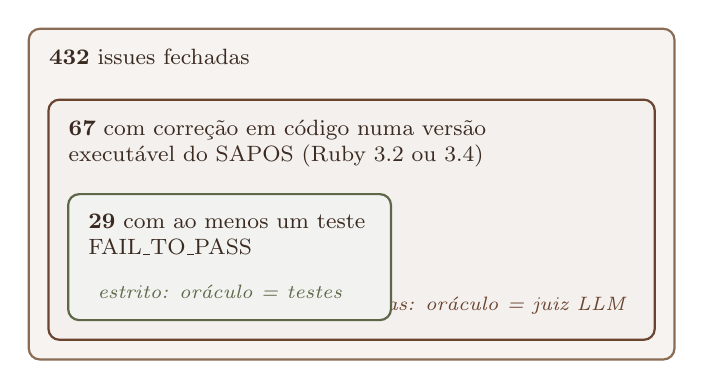
\begin{tikzpicture}[font=\footnotesize, text=tinta,
  conj/.style={draw=#1, line width=0.8pt, fill=#1!8, rounded corners=4pt},
  rot/.style={anchor=north west, align=left, inner sep=0pt}]
\draw[conj=gb] (0,0) rectangle (82mm,42mm);
\node[rot] at (2.5mm,39.5mm) {\textbf{432} issues fechadas};

\draw[conj=ga] (2.5mm,2.5mm) rectangle (79.5mm,33mm);
\node[rot] at (5mm,30.5mm) {\textbf{67} com correção em código numa versão\\executável do SAPOS (Ruby 3.2 ou 3.4)};
\node[anchor=south east, font=\scriptsize\itshape, text=ga] at (77mm,4.5mm) {todas: oráculo = juiz LLM};

\draw[conj=gc] (5mm,5mm) rectangle (46mm,21mm);
\node[rot] at (7.5mm,18.5mm) {\textbf{29} com ao menos um teste\\FAIL\_TO\_PASS};
\node[anchor=south west, font=\scriptsize\itshape, text=gc] at (7.5mm,6.5mm) {estrito: oráculo = testes};
\end{tikzpicture}
\end{document}
